

\section{Warping}
\label{sect:warping}

The key idea of this paper is that when transactions run
awry into an inconsistent state, rather than aborting them and
starting again from the beginning, it may be possible to
\emph{correct} the shared/local state directly by directly
modifying the state. Thus, the program continues as if it had not
gone down the bad path to the inconsistent state.
In this way we exploit a large design space, predicted by the \PMPY{}
model, but yet unexplored.

A thread $(c\times \lstack \times L)$ consists of code $c$, some local
stack $\lstack$ (for arguments and return values), and a local log
$L$. When executing a transaction, the code is of the form $\tx{c}$.
%
A given code $c$ induces a tree, with the root node labeled $c$. For
each $m$ and $c'$ such that $\step{c}{m}{c'}$, we create a child node
labled $c'$ and label the arc as $m$. If, for a node labeled $c$,
$\nothing{c}$ holds, then that note shall be a leaf.  We will
illustrate warping with the following example tree:
\begin{center}
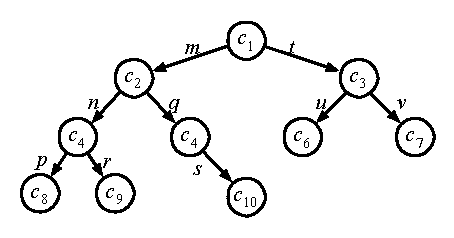
\includegraphics[width=2.8in]{stages0.eps}
\end{center}

\paragraph{Warping.}
The main idea of corrective synchronization is that transactions, in
instances of conflict, change their behavior to another possible
\red{more...}

Let us say, for example, that the example transaction has already
executed the following path:
\[\begin{array}{cl}
 (c_1,\lstack,[])\\
  \downarrow & \text{\APPLY}: \step{c_1}{m}{c_2} \text{ and } L'=L\cdot[m]\\
 (c_2,\lstack',[m])\\
  \downarrow & \text{\APPLY}: \step{c_2}{n}{c_4} \text{ and } L'=L\cdot[n]\\
 (c_4,\lstack'',[m,n])\\
\end{array}\]
% \begin{itemize*}
% \item From $(c_1,\lstack,[])$, $\step{c_1}{m}{c_2}$ holds, so \APPLY{}$(m)$.
% \item From $(c_2,\lstack',[m])$, $\step{c_2}{n}{c_4}$ holds, so \APPLY{}$(n)$.
% \item Ending at $(c_4,\lstack'',[m,n])$
% \end{itemize*}
For now, let us assume for simplicity that the transaction has not
\PUSH{}ed any of these methods.

At this stage, let us say that another transaction has committed. This
event may introduce conflict, either with one of the methods already
performed ($m$ or $n$) or with some/all of the methods in the subtree
of $c_4$: $p$ and $r$. When conflict is inevitable, standard
transactional memory implementations have no choice but to abort the
transaction and roll back to the original code $c_1$.

We observe that, in some cases, it may be more efficient to avoid the
process of aborting and restarting and instead, \emph{correcting}
behavior by transitioning directly to an alternate location on the
transaction tree, where the outlook is better. Consider this diagram:
\begin{center}
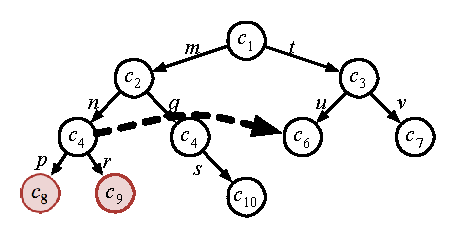
\includegraphics[width=2.8in]{stages1.eps}
\end{center}
Here the transaction has 

\paragraph{Correction.}

code\\
local state\\
log correction of $[n^{-1};m^{-1};t;u]$

\paragraph{Adding pessimistic behavior.}
%
The description thus far has been purely optimistic: a transaction
does not share its effects until it commits. A transaction may
\PUSH{} some of its effects to the shared log. However, this
constrains the transaction's warp destinations. 
%
If, in the running example, operation $m$ has been \PUSH{}ed, then it
is not possible for the transaction to warp to any node in the right
subtree of $c_1$. The transaction may, however, warp to node $c_4$,
applying a correction of $[n^{-1};q]$.
%
It is only possible for the transaction to warp to the right subtree
of $c_1$ if it first rolls backward, \UNPUSH{}ing $m$. This may
require global coordination if another transaction has already \PULL{}ed $m$.

\begin{theorem} The transition system is serializable.
\begin{proof}Via simulation with the \PMPY{} model~\cite{KP:PLDI15}.
\end{proof}
\end{theorem}

Being able to perform these warp operations depends crucially on a
few factors that we will explore in the rest of this paper:
\begin{itemize*}
\item Detecting when conflict is inevitable.
\item Detecting which warp destinations are possible and conflict-free.
\item How to correct: modifing the current local state, stack and
  program counter so that it
  is compatible with that alternate destination
\end{itemize*}
We address these issues with a combination of static and dynamic analysis.

\red{what about side effects?}

%%% Local Variables: 
%%% mode: latex
%%% TeX-master: "paper"
%%% End: 
